\documentclass[12pt, a4paper]{article}
\usepackage[a4paper, includeheadfoot, mag=1000, left=2cm, right=1.5cm, top=1.5cm, bottom=1.5cm, headsep=0.8cm, footskip=0.8cm]{geometry}
% Fonts
\usepackage{fontspec, unicode-math}
\setmainfont[Ligatures=TeX]{CMU Serif}
\setmonofont{CMU Typewriter Text}
\usepackage[english, russian]{babel}
% Indent first paragraph
\usepackage{indentfirst}
\setlength{\parskip}{5pt}
% Diagrams
\usepackage{graphicx}
\usepackage{float}
% Page headings
\usepackage{fancyhdr}

\usepackage{geometry}
\usepackage{array}

\pagestyle{fancy}
\renewcommand{\headrulewidth}{0pt}
\setlength{\headheight}{16pt}
%\newfontfamily\namefont[Scale=1.2]{Gloria Hallelujah}
\fancyhead{}

\usepackage{amsmath}

\graphicspath{ {images/} }

\usepackage{listings}
\lstdefinestyle{lablisting}{
  basicstyle=\scriptsize\ttfamily,
  numbers=left,
  stepnumber=1,
  otherkeywords={EOF, O\_RDONLY, STDIN\_FILENO, STDOUT\_FILENO, STDERR\_FILENO},
  numbersep=10pt,
  showspaces=false,
  showstringspaces=false
}

\newcommand{\specialcell}[2][l]{%
  \begin{tabular}[#1]{@{}l@{}}#2\end{tabular}}

\begin{document}

% Title page
\begin{titlepage}
\begin{center}

\textsc{Национальный исследовательский университет ИТМО\\[4mm]
Факультет программной инженерии и компьютерной техники}
\vfill
\textbf{Практическое задание №3\\[4mm]
по дисципение Теория Автоматов\\[4mm]
Канонический метод структурного синтеза\\[4mm]
}
\textit{Вариант 11\\[16mm]}
\begin{flushright}
Студент: Саржевский Иван
\\[2mm]Группа: P3302
\\[2mm]Преподаватель: Тропченко Александр Ювенальевич
\end{flushright}
\vfill
г. Санкт-Петербург\\[2mm]
2020 г.

\end{center}
\end{titlepage}

\section*{Цель}

Практическое освоение метода перехода от абстрактного автомата
к структурному автомату.

\section*{Задание}

Абстрактный автомат задан табличным способом. Причем абстрактный
автомат Мили представлен таблицами переходов и выходов, а абстрактный
автомат Мура - одной отмеченной таблицей переходов. Для синтеза
структурного автомата использовать функционально полную систему
логических элементов И, ИЛИ, НЕ и автомат Мура, обладающий полнотой
переходов и полнотой выходов. Синтезированный структурный автомат
представить в виде ПАМЯТИ и КОМБИНАЦИОННОЙ СХЕМЫ.

\section*{Исходные данные}

Согласно полученному варианту исходный автомат Мура задается
следующей таблицей переходов: 

\begin{center}
  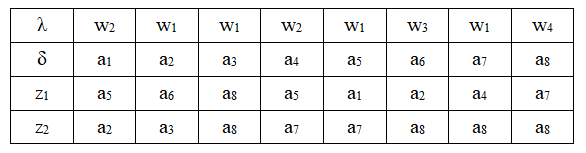
\includegraphics{task.png}
\end{center}

\section*{Кодирование исходного автомата двоичными кодами}

\subsection*{Входной алфавит}

\begin{tabular}{| c | c |}
  \hline
  & $x_1$\\
  \hline
  $z_1$ & \texttt{0}\\
  $z_2$ & \texttt{1}\\
  \hline
\end{tabular}

\subsection*{Выходной алфавит}

\begin{tabular}{| c | c | c |}
  \hline
  & $y_1$ & $y_2$\\
  \hline
  $w_1$ & \texttt{0} & \texttt{0}\\
  $w_2$ & \texttt{0} & \texttt{1}\\
  $w_3$ & \texttt{1} & \texttt{0}\\
  $w_4$ & \texttt{1} & \texttt{1}\\
  \hline
\end{tabular}

\subsection*{Состояния}

\begin{tabular}{| c | c | c | c |}
  \hline
  & $Q_1$ & $Q_2$ & $Q_3$\\
  \hline
  $a_1$ & \texttt{0} & \texttt{0} & \texttt{0}\\
  $a_2$ & \texttt{0} & \texttt{0} & \texttt{1}\\
  $a_3$ & \texttt{0} & \texttt{1} & \texttt{0}\\
  $a_4$ & \texttt{0} & \texttt{1} & \texttt{1}\\
  $a_5$ & \texttt{1} & \texttt{0} & \texttt{0}\\
  $a_6$ & \texttt{1} & \texttt{0} & \texttt{1}\\
  $a_7$ & \texttt{1} & \texttt{1} & \texttt{0}\\
  $a_8$ & \texttt{1} & \texttt{1} & \texttt{1}\\
  \hline
\end{tabular}

\section*{Таблицы переходов и выходов соответствующего структурного автомата}

После кодирования исходного абстрактного автомата
Мура построим таблицы переходов и выходов структурного автомата.

\begin{tabular}{|*{9}{c|}}
  \hline
  $x_1/Q_1Q_2Q_3$ & 000 & 001 & 010 & 011 & 100 & 101 & 110 & 111\\\hline
  0 & 100 & 101 & 111 & 100 & 000 & 001 & 011 & 110\\\hline
  1 & 001 & 010 & 111 & 110 & 110 & 111 & 111 & 111\\\hline
\end{tabular}

\begin{tabular}{|*{9}{c|}}
  \hline
  $x_1/Q_1Q_2Q_3$ & 000 & 001 & 010 & 011 & 100 & 101 & 110 & 111\\\hline
  0 & 01 & 00 & 00 & 01 & 00 & 10 & 00 & 11\\\hline
  1 & 01 & 00 & 00 & 01 & 00 & 10 & 00 & 11\\\hline
   & $y_1y_2$ & $y_1y_2$ & $y_1y_2$ & $y_1y_2$ & $y_1y_2$ & $y_1y_2$ & $y_1y_2$ & $y_1y_2$\\\hline
\end{tabular}

\section*{ДНФ для выходных сигналов}

По полученным таблицам построим ДНФ для каждого выходного сигнала:

\begin{align*}
  y_1 &= \bar{x_1}Q_1\bar{Q_2}Q_3 \lor \bar{x_1}Q_1Q_2Q_3 \lor x_1Q_1\bar{Q_2}Q_3 \lor x_1Q_1Q_2Q_3 = 5 \lor 7 \lor 13 \lor 15\\
  y_2 &= \bar{x_1}\bar{Q_1}\bar{Q_2}\bar{Q_3} \lor \bar{x_1}\bar{Q_1}Q_2Q_3 \lor \bar{x_1}Q_1Q_2Q_3 \lor x_1\bar{Q_1}\bar{Q_2}\bar{Q_3} \lor x_1\bar{Q_1}Q_2Q_3 \lor x_1Q_1Q_2Q_3\\
    &= 0 \lor 3 \lor 7 \lor 8 \lor 11 \lor 15
\end{align*}

\section*{Синтез автомата на D-триггерах}

С учетом закона функционирования D–триггера построим таблицу сигналов функций возбуждения:

\noindent
\begin{tabular}{|*{9}{c|}}
  \hline
  $x_1/Q_1Q_2Q_3$ & 000 & 001 & 010 & 011 & 100 & 101 & 110 & 111\\\hline
  0 & 100 & 101 & 111 & 100 & 000 & 001 & 011 & 110\\\hline
  1 & 001 & 010 & 111 & 110 & 110 & 111 & 111 & 111\\\hline
   & $D_1D_2D_3$ & $D_1D_2D_3$ & $D_1D_2D_3$ & $D_1D_2D_3$ & $D_1D_2D_3$ & $D_1D_2D_3$ & $D_1D_2D_3$ & $D_1D_2D_3$\\\hline
\end{tabular}

ДНФ для сигналов функций возбуждения:

\begin{align*}
  D_1 &= \bar{x_1}\bar{Q_1}\bar{Q_2}\bar{Q_3} \lor \bar{x_1}\bar{Q_1}\bar{Q_2}Q_3 \lor \bar{x_1}\bar{Q_1}Q_2\bar{Q_3} \lor \bar{x_1}\bar{Q_1}Q_2Q_3 \lor \bar{x_1}Q_1Q_2Q_3 \lor x_1\bar{Q_1}Q_2\bar{Q_3} \lor x_1\bar{Q_1}Q_2Q_3 \lor\\
  & \lor x_1Q_1\bar{Q_2}\bar{Q_3} \lor x_1Q_1\bar{Q_2}Q_3 \lor x_1Q_1Q_2\bar{Q_3} \lor x_1Q_1Q_2Q_3 =\\
  & = 0 \lor 1 \lor 2 \lor 3 \lor 7 \lor 10 \lor 11 \lor 12 \lor 13 \lor 14 \lor 15\\
  D_2 &= \bar{x_1}\bar{Q_1}Q_2\bar{Q_3} \lor \bar{x_1}Q_1Q_2\bar{Q_3} \lor \bar{x_1}Q_1Q_2Q_3 \lor x_1\bar{Q_1}\bar{Q_2}Q_3 \lor x_1\bar{Q_1}Q_2\bar{Q_3} \lor x_1\bar{Q_1}Q_2Q_3 \lor x_1Q_1\bar{Q_2}\bar{Q_3} \lor\\
  & \lor x_1Q_1\bar{Q_2}Q_3 \lor x_1Q_1Q_2\bar{Q_3} \lor x_1Q_1Q_2Q_3 = 2 \lor 6 \lor 7 \lor 9 \lor 10 \lor 11 \lor 12 \lor 13 \lor 14 \lor 15\\
  D_3 &= \bar{x_1}\bar{Q_1}\bar{Q_2}Q_3 \lor \bar{x_1}\bar{Q_1}Q_2\bar{Q_3} \lor \bar{x_1}Q_1\bar{Q_2}Q_3 \lor \bar{x_1}Q_1Q_2\bar{Q_3} \lor x_1\bar{Q_1}\bar{Q_2}\bar{Q_3} \lor x_1\bar{Q_1}Q_2\bar{Q_3} \lor \\
  & \lor x_1Q_1\bar{Q_2}Q_3 \lor x_1Q_1Q_2\bar{Q_3} \lor x_1Q_1Q_2Q_3 = 1 \lor 2 \lor 5 \lor 6 \lor 8 \lor 10 \lor 13 \lor 14 \lor 15
\end{align*}

\subsection*{Функциональная схема структурного автомата на D-триггерах}

\begin{center}
  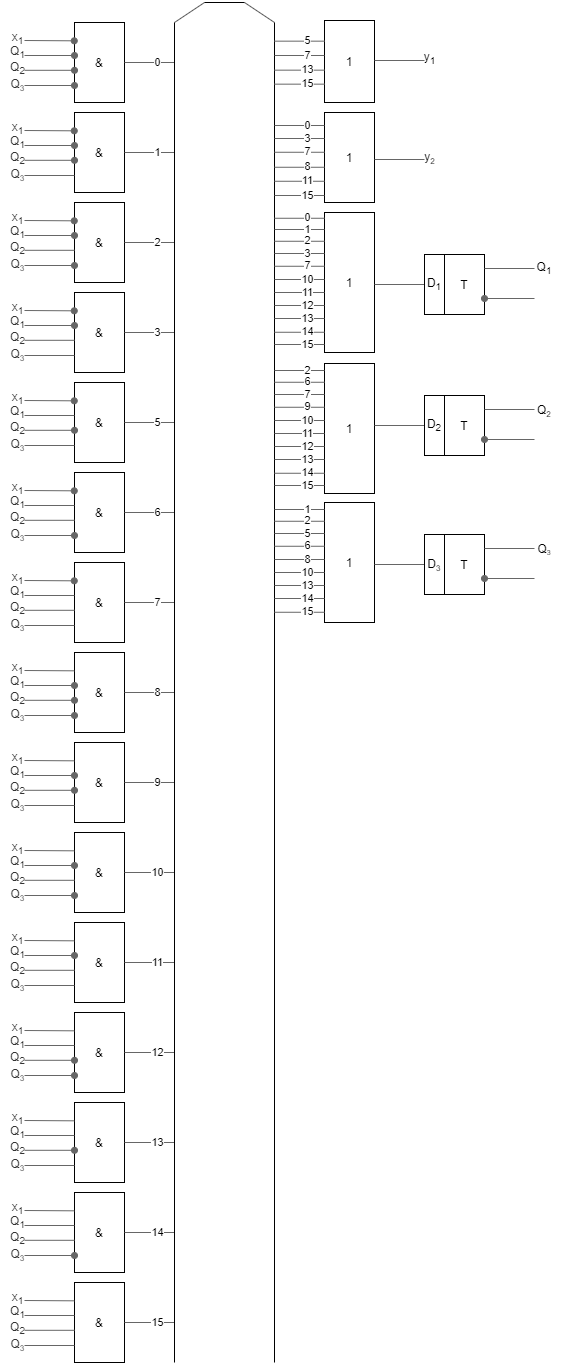
\includegraphics[scale=0.5]{d-trigger.png}
\end{center}

\subsection*{Тестирование функциональной схемы автомата}

\begin{center}
  \begin{tabular}{| l  l |}
    \hline
    Слово & \footnotesize{\texttt{1..0..0..1..0..1..0..1..0..0..0..0..0..1..0..1..0..0..0..1..0..1..0..0..0..0..1..1..1}}\\
    Ожид. & \footnotesize{\texttt{-- 00 10 00 00 11 11 00 11 00 01 00 01 00 00 01 00 01 00 01 00 10 11 00 01 00 01 00 00 11}}\\
    Резул. & \footnotesize{\texttt{-- 00 10 00 00 11 11 00 11 00 01 00 01 00 00 01 00 01 00 01 00 10 11 00 01 00 01 00 00 11}}\\\hline
  \end{tabular}
\end{center}

Результирующее слово совпадает с ожидаемым.

\section*{Синтез автомата на T-триггерах}

С учетом закона функционирования T–триггера построим таблицу сигналов функций возбуждения:

\begin{tabular}{|*{9}{c|}}
  \hline
  $x_1/Q_1Q_2Q_3$ & 000 & 001 & 010 & 011 & 100 & 101 & 110 & 111\\\hline
  0 & 100 & 100 & 101 & 111 & 100 & 100 & 101 & 001\\\hline
  1 & 001 & 011 & 101 & 101 & 010 & 010 & 001 & 000\\\hline
   & $T_1T_2T_3$ & $T_1T_2T_3$ & $T_1T_2T_3$ & $T_1T_2T_3$ & $T_1T_2T_3$ & $T_1T_2T_3$ & $T_1T_2T_3$ & $T_1T_2T_3$\\\hline
\end{tabular}

ДНФ для сигналов функций возбуждения:

\begin{align*}
  T_1 &= \bar{x_1}\bar{Q_1}\bar{Q_2}\bar{Q_3} \lor \bar{x_1}\bar{Q_1}\bar{Q_2}Q_3 \lor \bar{x_1}\bar{Q_1}Q_2\bar{Q_3} \lor \bar{x_1}\bar{Q_1}Q_2Q_3 \lor \bar{x_1}Q_1\bar{Q_2}\bar{Q_3} \lor \bar{x_1}Q_1\bar{Q_2}Q_3 \lor \bar{x_1}Q_1Q_2\bar{Q_3} \lor\\
  & \lor x_1\bar{Q_1}Q_2\bar{Q_3} \lor x_1\bar{Q_1}Q_2Q_3 = 0 \lor 1 \lor 2 \lor 3 \lor 4 \lor 5 \lor 6 \lor 10 \lor 11\\
  T_2 &= \bar{x_1}\bar{Q_1}Q_2Q_3 \lor x_1\bar{Q_1}\bar{Q_2}Q_3 \lor x_1Q_1\bar{Q_2}\bar{Q_3} \lor x_1Q_1\bar{Q_2}Q_3 = 3 \lor 9 \lor 12 \lor 13\\
  T_3 &= \bar{x_1}\bar{Q_1}Q_2\bar{Q_3} \lor \bar{x_1}\bar{Q_1}Q_2Q_3 \lor \bar{x_1}Q_1Q_2\bar{Q_3} \lor \bar{x_1}Q_1Q_2Q_3 \lor x_1\bar{Q_1}\bar{Q_2}\bar{Q_3} \lor x_1\bar{Q_1}\bar{Q_2}Q_3 \lor x_1\bar{Q_1}Q_2\bar{Q_3} \lor\\
  & \lor x_1\bar{Q_1}Q_2Q_3 \lor x_1Q_1Q_2\bar{Q_3} = 2 \lor 3 \lor 6 \lor 7 \lor 8 \lor 9 \lor 10 \lor 11 \lor 14
\end{align*}

\subsection*{Функциональная схема структурного автомата на T-триггерах}

\begin{center}
  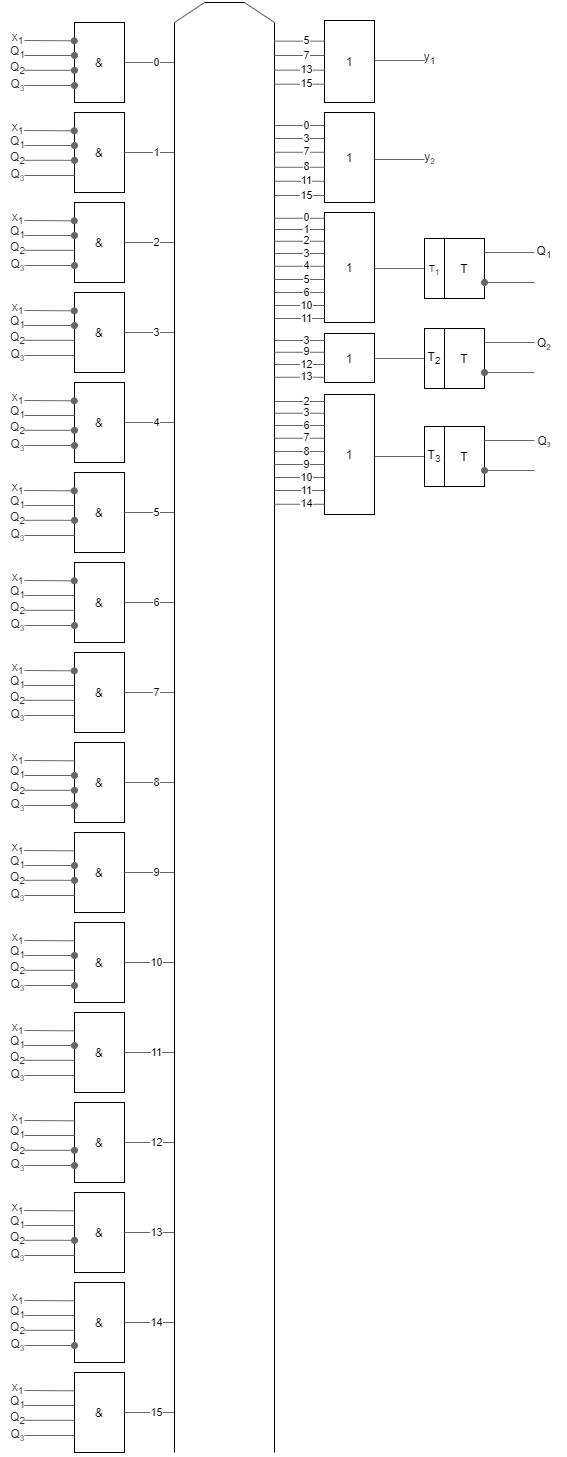
\includegraphics[scale=0.5]{t-trigger.png}
\end{center}

\subsection*{Тестирование функциональной схемы автомата}

\begin{center}
  \begin{tabular}{| l  l |}
    \hline
    Слово & \footnotesize{\texttt{1..0..0..1..0..1..0..1..0..0..0..0..0..1..0..1..0..0..0..1..0..1..0..0..0..0..1..1..1}}\\
    Ожид. & \footnotesize{\texttt{-- 00 10 00 00 11 11 00 11 00 01 00 01 00 00 01 00 01 00 01 00 10 11 00 01 00 01 00 00 11}}\\
    Резул. & \footnotesize{\texttt{-- 00 10 00 00 11 11 00 11 00 01 00 01 00 00 01 00 01 00 01 00 10 11 00 01 00 01 00 00 11}}\\\hline
  \end{tabular}
\end{center}

Результирующее слово совпадает с ожидаемым.

\section*{Синтез автомата на RS-триггерах}

С учетом закона функционирования RS–триггера построим таблицу сигналов функций возбуждения:

\noindent
\begin{footnotesize}
\begin{tabular}{|c|*{9}{>{\centering\arraybackslash}p{1.5cm}|}}
  \hline
  $x_1/Q_1Q_2Q_3$ & 000 & 001 & 010 & 011 & 100 & 101 & 110 & 111\\\hline
  0 & 01/-0/-0 & 01/-0/0- & 01/0-/01 & 01/10/10 & 10/-0/-0 & 10/-0/0- & 10/0-/01 & 0-/0-/10\\\hline
  1 & -0/-0/01 & -0/01/10 & 01/0-/01 & 01/0-/10 & 0-/01/-0 & 0-/01/0- & 0-/0-/01 & 0-/0-/0-\\\hline
   & $R_1S_1$/ $R_2S_2$/ $R_3S_3$ & $R_1S_1$/ $R_2S_2$/ $R_3S_3$ & $R_1S_1$/ $R_2S_2$/ $R_3S_3$ & $R_1S_1$/ $R_2S_2$/ $R_3S_3$ & $R_1S_1$/ $R_2S_2$/ $R_3S_3$ & $R_1S_1$/ $R_2S_2$/ $R_3S_3$ & $R_1S_1$/ $R_2S_2$/ $R_3S_3$ & $R_1S_1$/ $R_2S_2$/ $R_3S_3$\\\hline
\end{tabular}
\end{footnotesize}

ДНФ для сигналов функций возбуждения:

\begin{align*}
  R_1 &= \bar{x_1}Q_1\bar{Q_2}\bar{Q_3} \lor \bar{x_1}Q_1\bar{Q_2}Q_3 \lor \bar{x_1}Q_1Q_2\bar{Q_3} = 4 \lor 5 \lor 6\\
  S_1 &= \bar{x_1}\bar{Q_1}\bar{Q_2}\bar{Q_3} \lor \bar{x_1}\bar{Q_1}\bar{Q_2}Q_3 \lor \bar{x_1}\bar{Q_1}Q_2\bar{Q_3} \lor \bar{x_1}\bar{Q_1}Q_2Q_3 \lor x_1\bar{Q_1}Q_2\bar{Q_3} \lor x_1\bar{Q_1}Q_2Q_3 =\\
  &= 0 \lor 1 \lor 2 \lor 3 \lor 10 \lor 11\\
  R_2 &= \bar{x_1}\bar{Q_1}Q_2Q_3 = 3\\
  S_2 &= x_1\bar{Q_1}\bar{Q_2}Q_3 \lor x_1Q_1\bar{Q_2}\bar{Q_3} \lor x_1Q_1\bar{Q_2}Q_3 = 9 \lor 12 \lor 13\\
  R_3 &= \bar{x_1}\bar{Q_1}Q_2Q_3 \lor \bar{x_1}Q_1Q_2Q_3 \lor x_1\bar{Q_1}\bar{Q_2}Q_3 \lor x_1\bar{Q_1}Q_2Q_3 = 3 \lor 7 \lor 9 \lor 11\\
  S_3 &= \bar{x_1}\bar{Q_1}Q_2\bar{Q_3} \lor \bar{x_1}Q_1Q_2\bar{Q_3} \lor x_1\bar{Q_1}\bar{Q_2}\bar{Q_3} \lor x_1\bar{Q_1}Q_2\bar{Q_3} \lor x_1Q_1Q_2\bar{Q_3} = 2 \lor 6 \lor 8 \lor 10 \lor 14
\end{align*}

\subsection*{Функциональная схема структурного автомата на RS-триггерах}

\begin{center}
  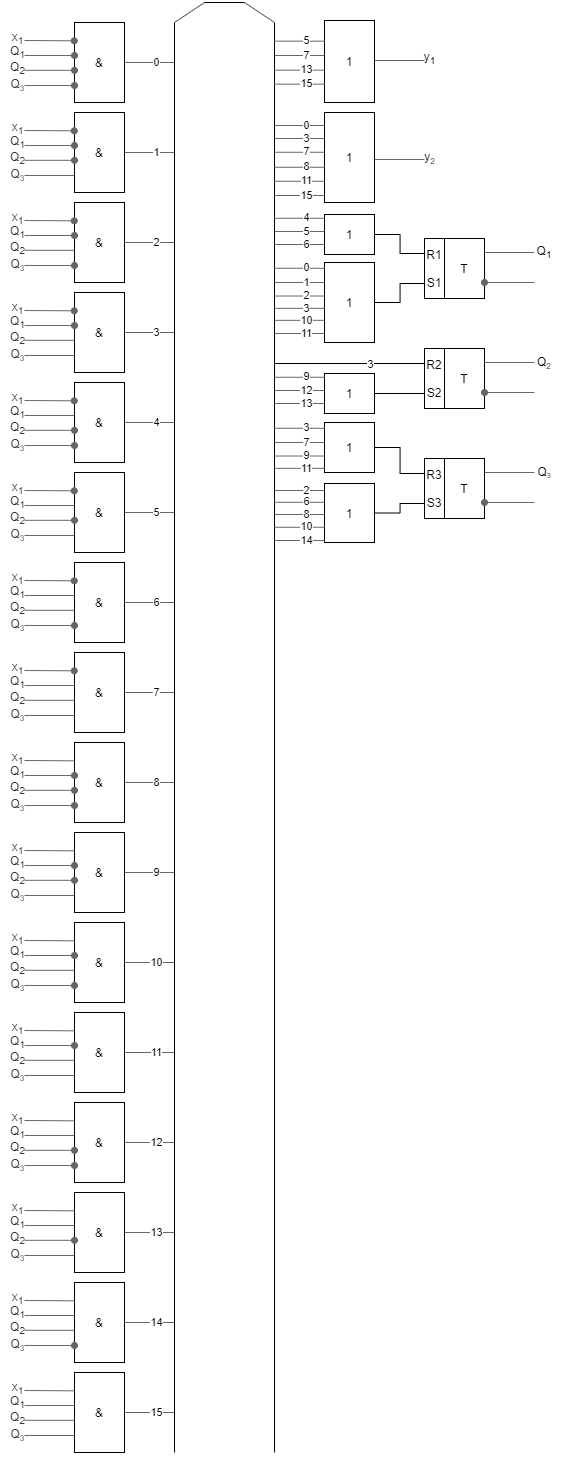
\includegraphics[scale=0.5]{rs-trigger.png}
\end{center}

\subsection*{Тестирование функциональной схемы автомата}

\begin{center}
  \begin{tabular}{| l  l |}
    \hline
    Слово & \footnotesize{\texttt{1..0..0..1..0..1..0..1..0..0..0..0..0..1..0..1..0..0..0..1..0..1..0..0..0..0..1..1..1}}\\
    Ожид. & \footnotesize{\texttt{-- 00 10 00 00 11 11 00 11 00 01 00 01 00 00 01 00 01 00 01 00 10 11 00 01 00 01 00 00 11}}\\
    Резул. & \footnotesize{\texttt{-- 00 10 00 00 11 11 00 11 00 01 00 01 00 00 01 00 01 00 01 00 10 11 00 01 00 01 00 00 11}}\\\hline
  \end{tabular}
\end{center}

Результирующее слово совпадает с ожидаемым.

\section*{Синтез автомата на JK-триггерах}

С учетом закона функционирования JK–триггера построим таблицу сигналов функций возбуждения:

\noindent
\begin{tabular}{|c|*{9}{>{\centering\arraybackslash}p{1.5cm}|}}
  \hline
  $x_1/Q_1Q_2Q_3$ & 000 & 001 & 010 & 011 & 100 & 101 & 110 & 111\\\hline
  0 & 1-/0-/0- & 1-/0-/-0 & 1-/-0/1- & 1-/-1/-1 & -1/0-/0- & -1/0-/-0 & -1/-0/1- & -0/-0/-1\\\hline
  1 & 0-/0-/1- & 0-/1-/-1 & 1-/-0/1- & 1-/-0/-1 & -0/1-/0- & -0/1-/-0 & -0/-0/1- & -0/-0/-0\\\hline
   & $J_1K_1$/ $J_2K_2$/ $J_3K_3$ & $J_1K_1$/ $J_2K_2$/ $J_3K_3$ & $J_1K_1$/ $J_2K_2$/ $J_3K_3$ & $J_1K_1$/ $J_2K_2$/ $J_3K_3$ & $J_1K_1$/ $J_2K_2$/ $J_3K_3$ & $J_1K_1$/ $J_2K_2$/ $J_3K_3$ & $J_1K_1$/ $J_2K_2$/ $J_3K_3$ & $J_1K_1$/ $J_2K_2$/ $J_3K_3$\\\hline
\end{tabular}

ДНФ для сигналов функций возбуждения:

\begin{align*}
  J_1 &= \bar{x_1}\bar{Q_1}\bar{Q_2}\bar{Q_3} \lor \bar{x_1}\bar{Q_1}\bar{Q_2}Q_3 \lor \bar{x_1}\bar{Q_1}Q_2\bar{Q_3} \lor \bar{x_1}\bar{Q_1}Q_2Q_3 \lor x_1\bar{Q_1}Q_2\bar{Q_3} \lor x_1\bar{Q_1}Q_2Q_3 =\\
  &= 0 \lor 1 \lor 2 \lor 3 \lor 10 \lor 11\\
  K_1 &= \bar{x_1}Q_1\bar{Q_2}\bar{Q_3} \lor \bar{x_1}Q_1\bar{Q_2}Q_3 \lor \bar{x_1}Q_1Q_2\bar{Q_3} = 4 \lor 5 \lor 6\\
  J_2 &= x_1\bar{Q_1}\bar{Q_2}Q_3 \lor x_1Q_1\bar{Q_2}\bar{Q_3} \lor x_1Q_1\bar{Q_2}Q_3 = 9 \lor 12 \lor 13\\
  K_2 &= \bar{x_1}\bar{Q_1}Q_2Q_3 = 3\\
  J_3 &= \bar{x_1}\bar{Q_1}Q_2\bar{Q_3} \lor \bar{x_1}Q_1Q_2\bar{Q_3} \lor x_1\bar{Q_1}\bar{Q_2}\bar{Q_3} \lor x_1\bar{Q_1}Q_2\bar{Q_3} \lor x_1Q_1Q_2\bar{Q_3} = 2 \lor 6 \lor 8 \lor 10 \lor 14\\
  K_3 &= \bar{x_1}\bar{Q_1}Q_2Q_3 \lor \bar{x_1}Q_1Q_2Q_3 \lor x_1\bar{Q_1}\bar{Q_2}Q_3 \lor x_1\bar{Q_1}Q_2Q_3 = 3 \lor 7 \lor 9 \lor 11
\end{align*}

\subsection*{Функциональная схема структурного автомата на JK-триггерах}

TODO: нарисовать

\subsection*{Тестирование функциональной схемы автомата}

\begin{center}
  \begin{tabular}{| l  l |}
    \hline
    Слово & \footnotesize{\texttt{1..0..0..1..0..1..0..1..0..0..0..0..0..1..0..1..0..0..0..1..0..1..0..0..0..0..1..1..1}}\\
    Ожид. & \footnotesize{\texttt{-- 00 10 00 00 11 11 00 11 00 01 00 01 00 00 01 00 01 00 01 00 10 11 00 01 00 01 00 00 11}}\\
    Резул. & \footnotesize{\texttt{-- 00 10 00 00 11 11 00 11 00 01 00 01 00 00 01 00 01 00 01 00 10 11 00 01 00 01 00 00 11}}\\\hline
  \end{tabular}
\end{center}

Результирующее слово совпадает с ожидаемым.

\section*{Вывод}

В ходе выполнения работы был изучен канонический метод структурного синтеза,
получены практические навыки преобразования абстрактного автомата Мура в
структурный автомат на D-, T-, RS- и JK-триггерах.

\end{document}
